\documentclass[11pt]{article}
\usepackage{paper_style}
\usepackage{graphicx} % Required for inserting images
\usepackage{indentfirst}
\usepackage{lipsum}
\usepackage{array}
\usepackage{float}
\usepackage{longtable}
\usepackage{enumitem}
\usepackage{hyperref}
\usepackage{float}
\usepackage{censor}
\usepackage{cleveref}
\usepackage{amsmath}
\usepackage[section]{minted}

%% ===============================================
%% Setting the line spacing (3 options: only pick one)
% \doublespacing
% \singlespacing
\onehalfspacing
%% ===============================================

\setlength{\droptitle}{-5em} %% Don't touch

\crefname{section}{Section}{Sections}
\crefname{figure}{Figure}{Figures}

\newmintedfile[pythoncode]{python}{%
    fontfamily=tt,
    linenos=true,
    breaklines=true,
    numberblanklines=true,
    numbersep=5pt,
    gobble=0,
    frame=leftline,
    framerule=0.4pt,
    framesep=2mm,
    funcnamehighlighting=true,
    tabsize=2,
    obeytabs=false,
    mathescape=false
    samepage=false, %with this setting you can force the list to appear on the same page
    showspaces=false,
    showtabs=false,
    texcl=false,
}

\begin{document}

%TC:ignore
\begin{titlepage}
    \begin{center}
        \null
        \vfill
            
        \Large
        \textbf{Predictive Modeling of Car Accident Severity in the USA from 2016-2023 using Machine Learning Techniques}
            
        \vspace{1.5cm}
        
        \large
        \censor{Saptak Das}
        
        November 2023
        
        \vfill
    \end{center}
\end{titlepage}
%TC:endignore

\section{Introduction}
\label{section:introduction}
As a student, who got their driver's license only a few months ago, I am eager, yet cautious to drive. Since I learned that teen drivers have a fatal crash rate almost three times as high as drivers ages 20 and older per mile driven (CDC), I try to keep my driving to a minimum. However, avoiding driving completely is not a practical solution. Being able to drive is an integral skill of our society. Moreover, to drive safely, experience is necessary, experience that I would lack by avoiding driving entirely.

Thus, to limit my driving risk, I have decided to derive a mathematical model to evaluate and advise me on the risk of driving in various driving scenarios. Through this mathematical model, I hope to understand the risks of driving more thoroughly in order to be safer and have more peace of mind when I am on the road. 

This IA will also significantly extend my mathematical understanding of how advanced statistics, linear algebra, and multivariable calculus can be used to understand and visualize trends in data, determine the most important features through dimensionality reduction, and create an accurate and applicable Machine Learning model to evaluate the driving risk of a particular situation.


\subsection{Research Question}
What conditions result in the most dangerous driving accidents?

\section{Dataset Overview}
Throughout this paper, I will be using the US Accidents (2016 - 2023) Dataset \citep{sobhanmoosavi_2023}. Before starting any analysis, it is essential to understand what data is provided. The data columns are described in \cref{section:traffic_attrs}, \cref{section:address_attrs}, \cref{section:weather_attrs}, \cref{section:poi_attrs}, and \cref{section:pod_attrs}. All data processing, analysis, and visualization are performed in Python \cref{code:python}.

\section{Data Cleaning and Preprocessing}
\noindent
Before analyzing this dataset, it must be cleaned and processed in order to derive accurate insights and predictive models.

\subsection{Reporting Sources}
\noindent
The data was compiled from two sources, Bing and MapQuest. These sources report severity differently, thus I had to decide which source to utilize. 

\begin{figure}[H]
    \centering
    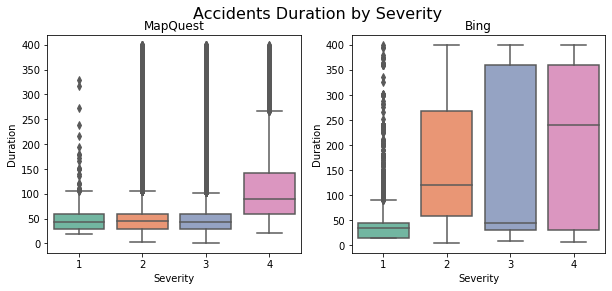
\includegraphics[width=115mm,height=\textheight,keepaspectratio]{images/duration_severity.png}
    \caption{Accident Duration by Severity}
    \label{fig:duration_severity}
\end{figure}

\begin{figure}[H]
    \centering
    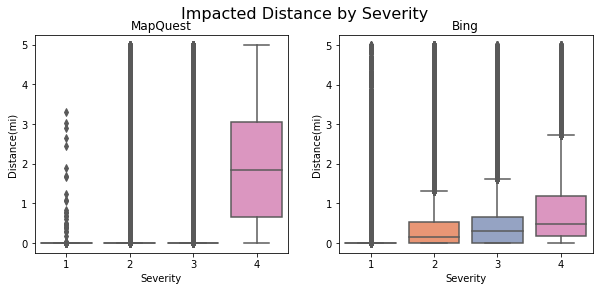
\includegraphics[width=115mm,height=\textheight,keepaspectratio]{images/distance_severity.png}
    \caption{Impacted Distance by Severity}
    \label{fig:distance_severity}
\end{figure}

As can be seen by \cref{fig:duration_severity,fig:distance_severity}, MapQuest has a clearly higher quartile 1, quartile 2 (median), and quartile 3 for severity 4. Bing seems to have a looser definition as the box and whisker plots are not too statistically significant from each other. For these reasons, I decided to only utilize the MapQuest data.

\subsection{Non-Predictive Features}
Data for columns 'ID', 'Distance(mi)', 'End Time', 'Duration', 'End Latitude', and 'End Longitude' can only be collected after the accident has already happened and hence cannot be used to predict severe accidents. Furthermore, since categorical variables like 'Country' and 'Turning Loop' only have one class, they cannot be predictive features as the probabilistic surprise and entropy for these random variables is 0 \citep{lesne2014shannon}.

\subsection{Filtering Incomplete Data}
Though this dataset is mostly complete, some entries lack data for certain columns. Rather than removing these columns for all entries, I decided to remove the incomplete row entries instead as the original dataset contains over 7.7 million accidents. Even after this filtering, there is still ample data.



\section{Understanding and Exploring Data}
\label{section:exploratory_analysis}

Based on \cref{fig:duration_severity,fig:distance_severity}, the MapQuest accidents with severity 4 are much more serious than other severity accidents. These other levels of severity are hard to distinguish from each other. Thus, I decided to focus on severity 4 accidents (from now referred to as "severe") and group the other severity accidents (from now referred to as "non-severe") together.

\subsection{Data Sample Normalization}
In this processed dataset, there are roughly 2.61 million non-severe accidents and only 9000 severe accidents. This discrepancy must be normalized before conducting any further exploratory analysis. I created a Python function to return a random sample of 50000 undersampled non-severe and 50000 oversampled severe accidents.

\subsection{Trends based on Time}
\noindent
Next, I decided to explore if there were trends based on time.

\begin{figure}[H]
    \centering
    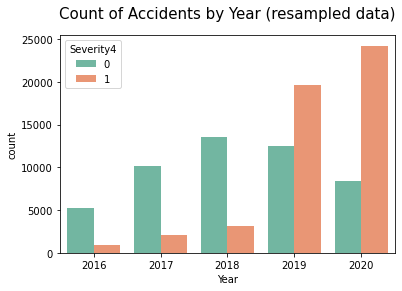
\includegraphics[width=80mm,height=\textheight,keepaspectratio]{images/accident_counts.png}
    \caption{Count of Accidents by Year}
    \label{fig:accidents_year}
\end{figure}

\noindent
Looking at Figure \ref{fig:accidents_year}, it is highly improbable that severe accidents rose by 5 times from 2018 to 2019. To investigate this, I created a heatmap of these severe accidents to see how the data is actually distributed.

\begin{figure}[H]
    \centering
    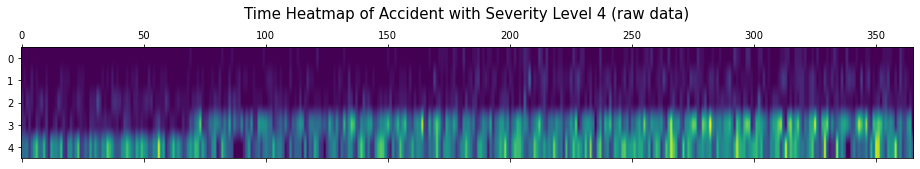
\includegraphics[width=130mm,height=\textheight,keepaspectratio]{images/severe_heatmap.png}
    \caption{Time Heatmap of Severe Accidents}
    \label{fig:severe_heatmap}
\end{figure}

This heatmap strongly indicates that something changed after February 2019, such as the way that MapQuest defines severity or the way they collected data. Since the data after February 2019 is consistent with data in the future, dropping the data before March 2019 is the best choice for analysis and predictions.

\subsection{Log Frequency Normalization}
Next, I decided to analyze the accidents per hour. In \cref{fig:counts_hour}, there are two clear peaks in non-severe accidents occurring at roughly at 7-8 am and 4-5 pm, which likely correlate to maximum traffic times due to work-home commutes.

\begin{figure}[H]
    \centering
    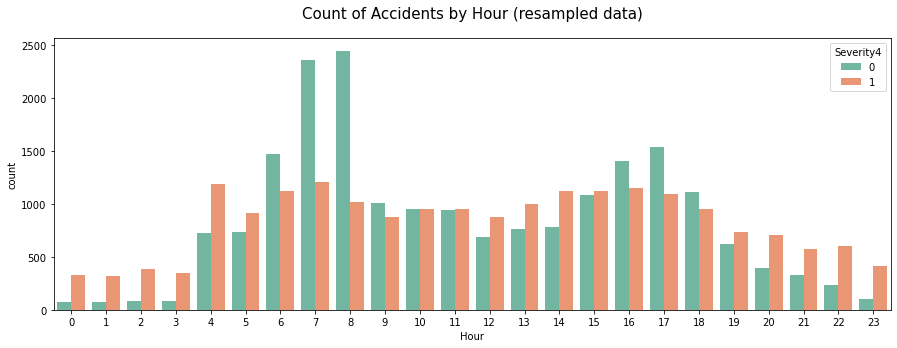
\includegraphics[width=130mm,height=\textheight,keepaspectratio]{images/count_hour.png}
    \caption{Count of Accidents by Hour}
    \label{fig:counts_hour}
\end{figure}

It is also interesting to note that during the hours (early morning or late night) where there were less non-severe accidents, there tended to be relatively greater severe accidents. This observation could be made clearer by using other data for a specific day, hour, or minute. 

Since there are too many classes for a categorical variable for hours, I took the frequency of accidents during the hour. However, since certain hours could have a relatively low frequency, while others could have a relatively high frequency, the log of the frequency is taken to normalize the random continuous variable into a Gaussian distribution. Just in case the frequency is 0, 1 is added to all frequencies before taking the logarithm to prevent undefined values. This log frequency normalization \citep{macurdypencavellog} is defined in Equation \ref{eq:log_freq}.

\begin{equation} \label{eq:log_freq}
    X = \log \left(\left({\frac{n_i}{\sum_{j}^{k}n_j}} \times N_u\right) + 1\right)
\end{equation}

\noindent
where:
\begin{itemize}
    \item $X$ is the resulting continuous random variable after normalization.
    \item $n_i$ is the number of times a possible class of a categorical variable occurs.
    \item $\sum_{j}^{k}n_j$ is the total number of samples.
    \item $N_u$ is the number of unique classes that the categorical variable can take.
\end{itemize}


\begin{table}[H] 
\centering
\begin{tabular}{lll}
Severe & Hour & Hour Freq \\ \hline
1      & 22   & 3         \\
0      & 14   & 2         \\
0      & 5    & 1         \\
0      & 22   & 3         \\
0      & 14   & 2         \\
1      & 22   & 3        
\end{tabular}
\caption{Example Data for Hour Log Frequency Normalization}
\label{table:log_freq}
\end{table}

\noindent
For example, using the example data in Table \ref{table:log_freq}, the hour log frequency normalization for the first row can be performed using Equation \ref{eq:log_freq_example}.

\begin{align} \label{eq:log_freq_example}
    X &= \log \left(\left({\frac{n_i}{\sum_{j}^{k}n_j}} \times N_u\right) + 1\right) \\
    &= \log \left(\left({\frac{3}{6}} \times 24 \right) + 1\right) \\
    &= \log 13 \approx 2.56
\end{align}

\begin{figure}[H]
    \centering
    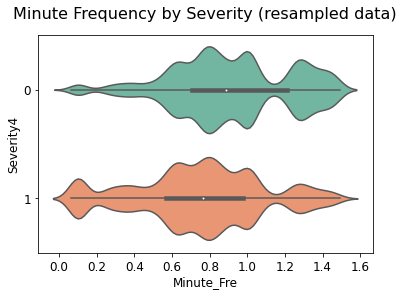
\includegraphics[width=80mm,height=\textheight,keepaspectratio]{images/violin_minute.png}
    \caption{Accidents by Location Frequency}
    \label{fig:violin_minute}
\end{figure}

\subsection{Location}
\cref{fig:violin_lat_lng} shows the distribution of accidents based on latitude and longitude. The violin plots for non-severe and severe accidents seem to be very similar, though there are subtle changes in the ratio of the types of accidents.

\begin{figure}[H]
    \centering
    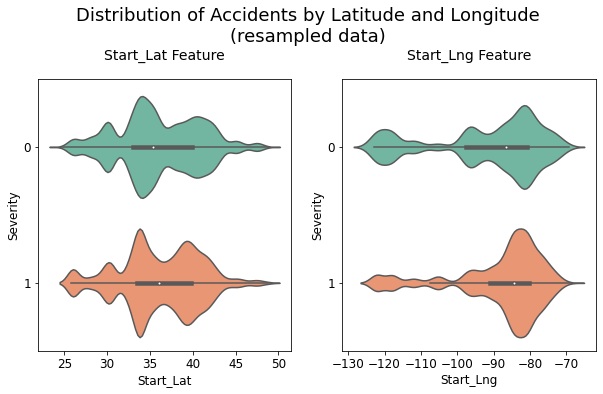
\includegraphics[width=100mm,height=\textheight,keepaspectratio]{images/violin_lat_lng.png}
    \caption{Accidents by Latitude and Longitude}
    \label{fig:violin_lat_lng}
\end{figure}

In \cref{fig:map_accidents}, I plotted the latitude and longitude. I was fascinated to see how clearly the accidents were distributed across the US. The figure clearly shows more densely populated areas tended to have more accidents. More interesting, however, was how the severe accidents seemed to most densely be located in network-like structure. This seemed to indicate the US interstate highway system was where the greatest number of accidents seemed to occur.

\begin{figure}[H]
    \centering
    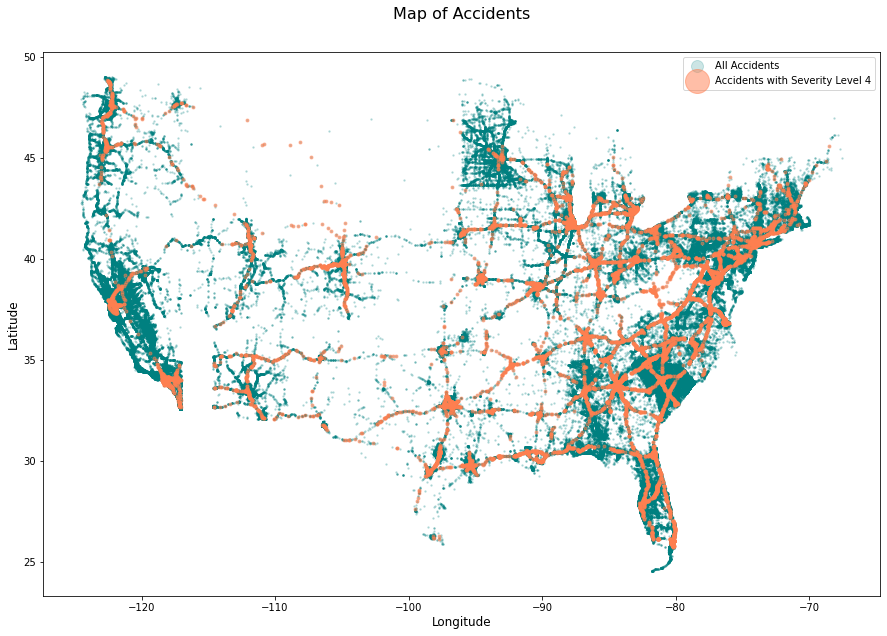
\includegraphics[width=115mm,height=\textheight,keepaspectratio]{images/map_accidents.png}
    \caption{Map of Accidents}
    \label{fig:map_accidents}
\end{figure}

Using Equation \ref{eq:log_freq}, I used the frequency of local indicators such as 'Street', 'City', 'County', 'Zipcode', 'Airport Code', and 'State' to try to capture the clear correlation to the highway accidents in continuous random variables.

\begin{figure}[H]
    \centering
    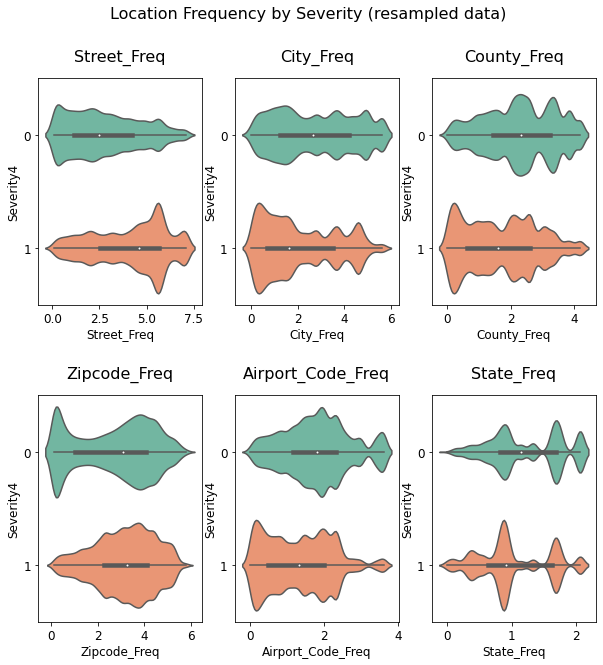
\includegraphics[width=100mm,height=\textheight,keepaspectratio]{images/violin_loc.png}
    \caption{Accidents by Location Frequency}
    \label{fig:violin_loc}
\end{figure}

\subsection{Weather Features}
Since the weather features such as 'Pressure', 'Visibility', and 'Wind Speed' are highly skewed, they must be normalized prior to analysis. A Box Cox transformation \citep{osborne2010improving} can turn non-normal dependent variables into a normal Gaussian shape. By precisely controlling the parameter \(\lambda\), I was able to normalize the weather features.

\begin{equation} \label{eq:boxcox_transform}
    y(\lambda)=
    \begin{cases}
        \frac{y^\lambda - 1}{\lambda} & \lambda \neq 0 \\
        \log{y} & \lambda = 0
    \end{cases}
\end{equation}

Overall, \cref{fig:bar_weather} shows that accidents are little more likely to be serious during rain or snow while less likely on a cloudy day.

\begin{figure}[H]
    \centering
    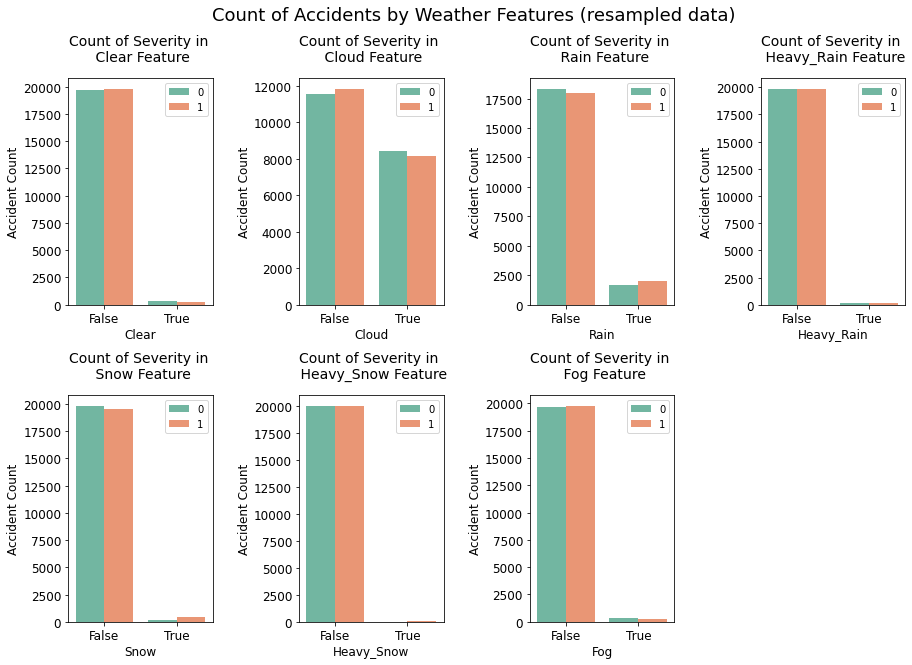
\includegraphics[width=100mm,height=\textheight,keepaspectratio]{images/bar_weather.png}
    \caption{Accidents by Weather}
    \label{fig:bar_weather}
\end{figure}

\section{Point of Interest Features}
\noindent
\cref{fig:accidents_poi} shows the number of accidents that occurred at Points of Interest (POI).

\begin{figure}[H]
    \centering
    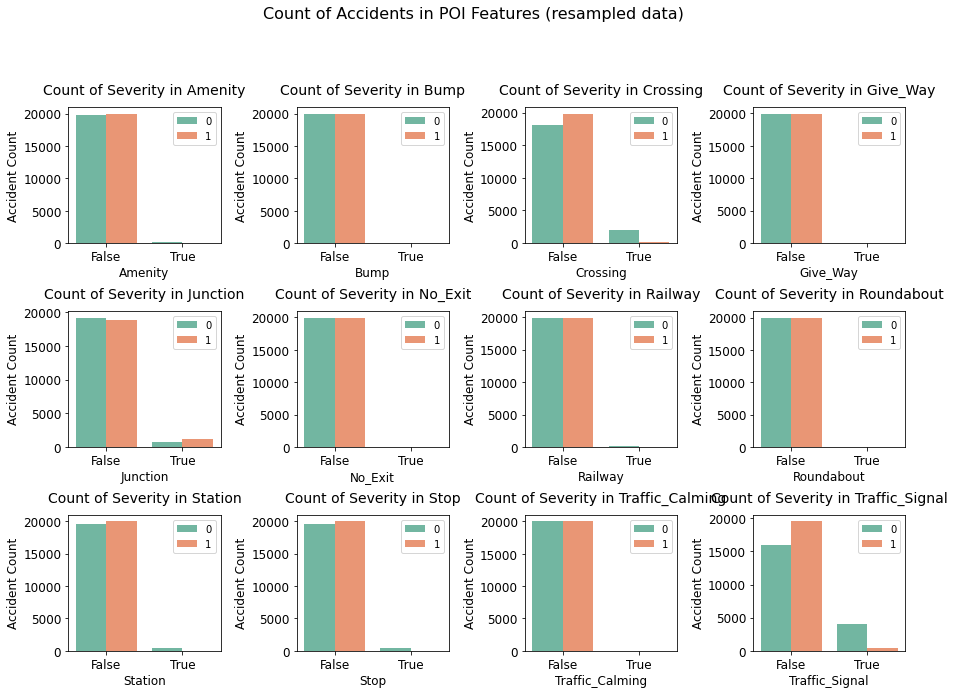
\includegraphics[width=130mm,height=\textheight,keepaspectratio]{images/accidents_poi.png}
    \caption{Accidents by Location Frequency}
    \label{fig:accidents_poi}
\end{figure}

Accidents near traffic signal and crossing are much less likely to be serious accidents while little more likely to be serious if they are near the junction. This may occur because drivers usually slow down in front of crossing and traffic signal but junction and severity are highly related to speed. The other POI features have such little severe accidents that it is hard to tell their relation with severity from plots.

\subsection{Heatmap Correlation}
After all the normalization and processing performed, the following correlation heatmap was derived.

\begin{figure}[H]
    \centering
    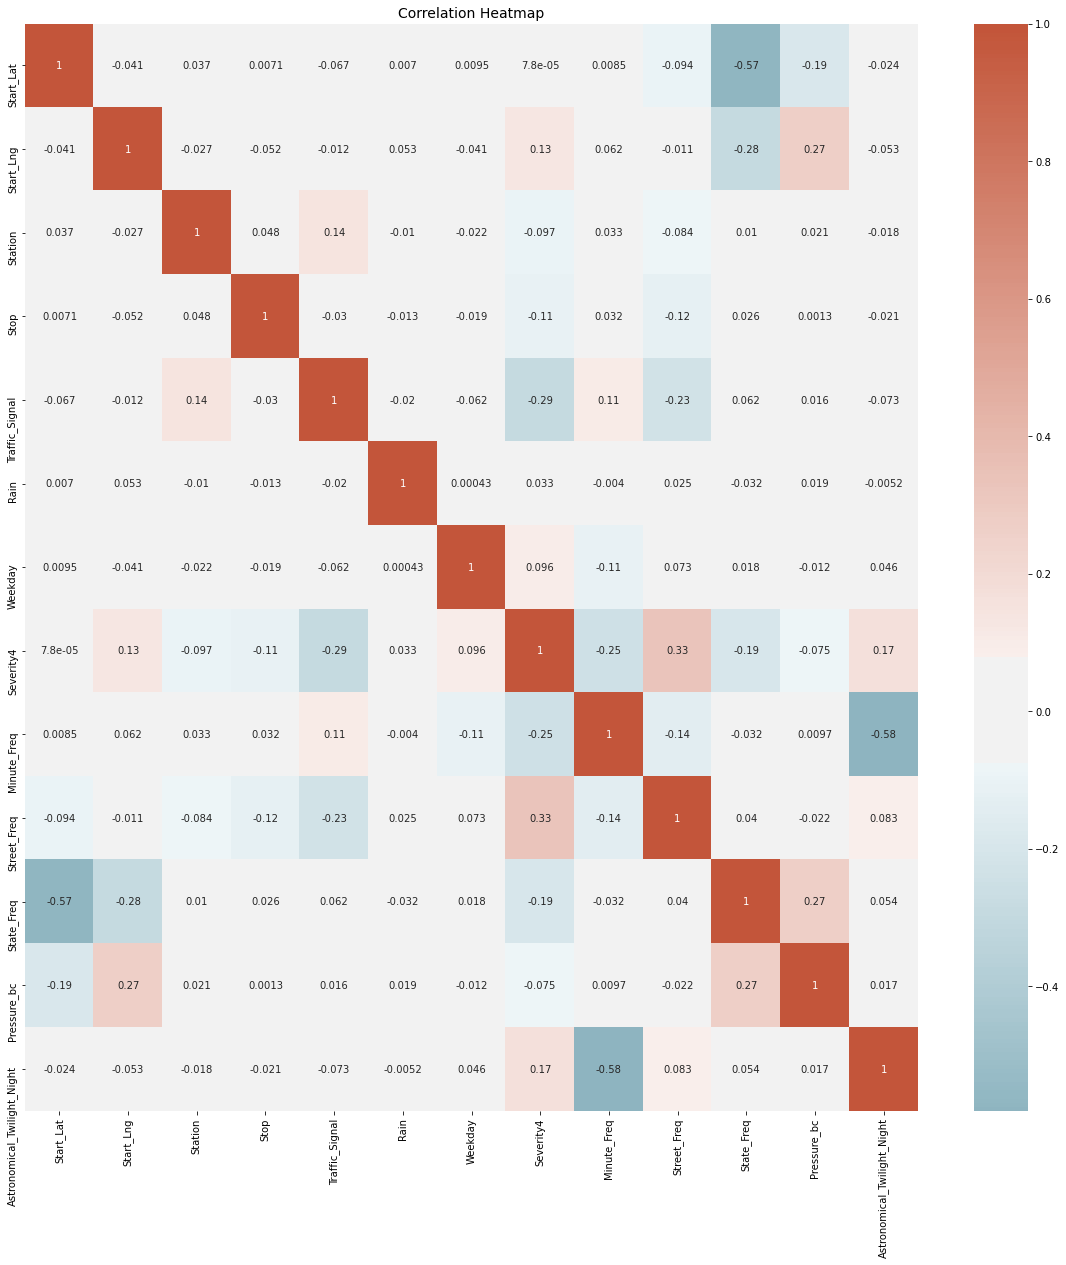
\includegraphics[width=80mm,height=\textheight,keepaspectratio]{images/corr_heatmap.png}
    \caption{Correlation Heatmap}
    \label{fig:corr_heatmap}
\end{figure}

\noindent
This heatmap represents the Pearson correlation coefficient (Equation \ref{eq:correlation_coefficient}) for each pair of continuous random variables in the dataset.

\begin{equation} \label{eq:correlation_coefficient}
    r = \frac{N\sum{XY}-(\sum{X}\sum{Y})}{\sqrt{ [N \sum{x^2}-(\sum{x})^2 ][N \sum{y^2}-(\sum{y})^2 }]}
\end{equation}

The Correlation Heatmap is promising as it shows both mildly strong positive and negative correlations of the various data columns to the severity, while being minimally correlated to each other. 

This should in theory should enable enable a predictive model to optimize weights of select factors in order to derive a strong fit.

\section{Predictive Modeling}
\noindent
Using the processed data from \cref{section:exploratory_analysis}, I finally could start on designing a predictive model.

\subsection{Principal Component Analysis}
Even though I had majorly reduced the dimensionality of the data from 48 columns to only 12 columns through the processing steps, this was still too much data to pass into a predictive model. As a result, I decided to use Principal Component Analysis (PCA), which reduces data dimensionality while retaining most of the relevant information.

\noindent
\newline
PCA involves:
\begin{enumerate}
    \item Centering the data about the origin.
    \begin{itemize}
        \item \(X'_i = X_i - \bar{X}\)
    \end{itemize}
    \item Calculating the covariance matrix with n variables.
    \begin{itemize}
        \item \(Cov(X, Y) = \frac{1}{n-1} \sum_{i=1}^{n} \left(X'_i-\bar{X}\right) \left(Y'_i-\bar{Y}\right) \)
    \end{itemize}
    \item Compute the eigenvalues \(\lambda\) and eigenvectors \(v\) of the covariance matrix \(C\).
    \begin{itemize}
        \item \(Cv = \lambda v\)
    \end{itemize}
    \item Selecting the top \(k\) principal component eigenvalues and corresponding eigenvectors.
    \item Projecting an original point (X) onto the new feature space along the ith principle component \(v_i\).
    \begin{itemize}
        \item \(X' = X \dot v_i\)
    \end{itemize}
    \item The principal components are linear combinations of the original variables. \(a_{ij}\) represents the components of the ith eigenvector. This represents the general form for the principal component i.
    \begin{itemize}
        \item \(PC_i = a_{i1} X'_1 + a_{i2} X'_2 + \dots + a_{in} X'_n\)
    \end{itemize}
\end{enumerate}

\noindent
After performing PCA, the explained variance ratio can be derived using the Equation \ref{eq:explained_variance}. Using PC1, PC2, ..., and PC8, over 80\% of the variance in the accident severity is captured. This is described in the Scree Plot in \cref{fig:scree_plot}.

\begin{equation} \label{eq:explained_variance}
    \text{Explained Variance} = \frac{\lambda_i}{\lambda_1 + \lambda_2 + \dots +\lambda_n}
\end{equation}

\begin{figure}[H]
    \centering
    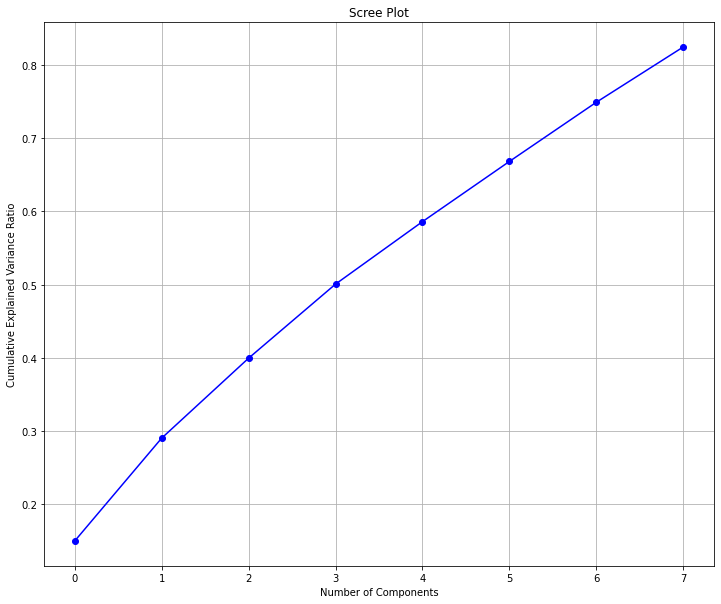
\includegraphics[width=100mm,height=\textheight,keepaspectratio]{images/scree_plot.png}
    \caption{Scree Plot}
    \label{fig:scree_plot}
\end{figure}

\subsection{Binary Logisitic Regression}
\label{section:logistic_regression}
In order to prevent overfitting and address the bias-variance tradeoff \citep{belkin2019reconciling}, I split the data into 80\% training and 20\% testing. Using the PCs derived in the previous step, I decided to try using a binary logistic regression.

\noindent
\newline
A binary logistic regression is defined by Equation \ref{eq:logistic_regression}.
\begin{equation} \label{eq:logistic_regression}
    y=\frac{1}{1+e^{-\left(\beta_0 + \beta_1 x \right)}}
\end{equation}

To tune the parameters \(\beta_0\) and \(\beta_1\), a maximum likelihood interpretation is utilized. Equation \ref{eq:joint_likelihood} describes the calculation for joint likelihood \(L(\beta_0, \beta)\).
\begin{equation} \label{eq:joint_likelihood}
    L(\beta_0, \beta) = \prod_{i=1}^{n} \left(p(x_i)\right)^{y_i} \times \left(1-p(x_i)\right)^{1 - y_i} 
\end{equation}

\noindent
This can further be simplified by taking the log-likelihood \(l(\beta_0, \beta)\) described in Equation \ref{eq:log_joint_likelihood}
\begin{equation} \label{eq:log_joint_likelihood}
    l(\beta_0, \beta) = \sum_{i=1}^{n} y_i \log \left(p(x_i)\right) + \left(1 - y_i\right) \log \left(1-p(x_i)\right) 
\end{equation}

\noindent
After taking the partial derivative of the log-likelihood\(l(\beta_0, \beta)\) with respect to \(\beta_0\) and \(\beta\) parameters individually and simplifying, Equation \ref{eq:log_gradient} describes the gradient of the \(\beta_0\) and \(\beta_1\). By numerically stepping the \(\beta_0\) and \(\beta_1\) using the gradient from Equation \ref{eq:log_gradient}, the likelihood that the data was derived from the fitted logistic regression is maximized \citep{menard2002applied}.

\begin{equation} \label{eq:log_gradient}
    \frac{\partial l}{\partial \beta_j} = - \sum_{i=1}^{n} \left( y_i - p\left(x_i; \beta_0, \beta\right) \right) x_{ij}
\end{equation}

\subsubsection{Results}
\begin{figure}[H]
    \centering
    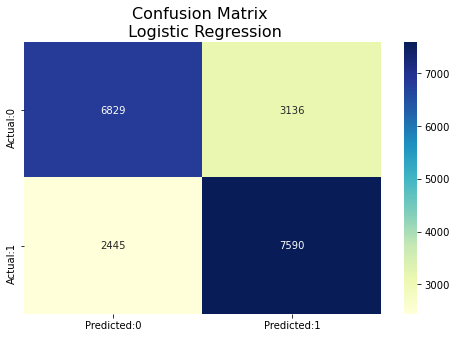
\includegraphics[width=90mm,height=\textheight,keepaspectratio]{images/log_conf_matrix.png}
    \caption{Logistic Regression Confusion Matrix}
    \label{fig:log_conf_matrix}
\end{figure}

\noindent
Using \cref{fig:log_conf_matrix} and Equations \ref{eq:sensitivity}, \ref{eq:specificity}, and \ref{eq:accuracy}, I calculated the sensitivity, specificity, and accuracy of my model.

\begin{align}
    \text{Sensitivity} &= \frac{TP}{TP + FN} \\ \label{eq:sensitivity}
    &= \frac{7590}{7590 + 2445} \\
    &\approx 75.6\% \\
    \text{Specificity} &= \frac{TN}{TN + FP} \\ \label{eq:specificity}
    &= \frac{6829}{6829 + 3136} \\
    &\approx 68.5\% \\
    \text{Accuracy} &= \frac{TP + TN}{TP + FP + FN + TN} \\ \label{eq:accuracy}
    &= \frac{7590 + 6829}{7590 + 3136 + 2445 + 6829} \\
    &\approx 72.1\% 
\end{align}
\noindent
where:
\begin{itemize}
    \item $TP$ is the number of True Positives.
    \item $TN$ is the number of True Negatives.
    \item $FP$ is the number of False Positives.
    \item $FN$ is the number of False Negatives.
\end{itemize}

\noindent
As can be seen in Equations \ref{eq:sensitivity}, \ref{eq:specificity}, and \ref{eq:accuracy}, the model has a relatively low sensitivity, specificity, and accuracy. I believe that a stronger predictive model can be created.

\subsection{Random Forest Classifier}
Given relatively weak results from \cref{section:logistic_regression}, I decided to try the more advanced Random Forest Classifier using GridSearchCV. Random Forest classifier is a machine learning model that combines the predictions of multiple decision trees to make more accurate and robust classifications. It works by creating a forest of decision trees, each trained on a random subset of the data and using a random subset of the features. The individual tree predictions are then aggregated to make the final classification decision, often through a majority vote or weighted average. Random Forests are known for their ability to handle high-dimensional data, reduce overfitting, and provide feature importance rankings, making them a popular choice for a wide range of classification tasks, from image recognition to financial risk assessment.

\subsubsection{Results}
\begin{figure}[H]
    \centering
    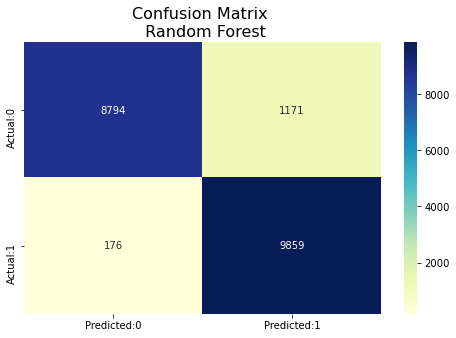
\includegraphics[width=90mm,height=\textheight,keepaspectratio]{images/rf_conf_matrix.png}
    \caption{Random Forest Confusion Matrix}
    \label{fig:rf_conf_matrix}
\end{figure}

\begin{align}
    \text{Sensitivity} &= \frac{TP}{TP + FN} \\ \label{eq:sensitivity2}
    &= \frac{9859}{9859 + 176} \\
    &\approx 98.2\% \\
    \text{Specificity} &= \frac{TN}{TN + FP} \\ \label{eq:specificity2}
    &= \frac{8794}{8794 + 1171} \\
    &\approx 88.2\% \\
    \text{Accuracy} &= \frac{TP + TN}{TP + FP + FN + TN} \\ \label{eq:accuracy2}
    &= \frac{9859 + 8794}{9859 + 1171 + 176 + 8794} \\
    &\approx 93.3\% 
\end{align}

\cref{fig:rf_conf_matrix} and Equations \ref{eq:sensitivity2}, \ref{eq:specificity2}, and \ref{eq:accuracy2} clearly show that the Random Forest Model is more sensitive, specific, and accurate than the Logisitic Model in \cref{section:logistic_regression}. Since the sensitivity (true positive rate) is \(98\%\) and the specificity (true negative rate) is \(88\%\), the Random Forest Classifier seems to miscategorize more non-severe accidents as severe \citep{zhu2010sensitivity}. This is acceptable for the practical application of this model as overestimating the severity of accidents would bring greater public awareness of dangerous driving conditions.

\section{Conclusion}
The most accurate predictive model that I created was the Random Forest Classifier with a 93\%. \cref{fig:rf_features} shows the most significant feature weights that the model iteratively learned.

\begin{figure}[H]
    \centering
    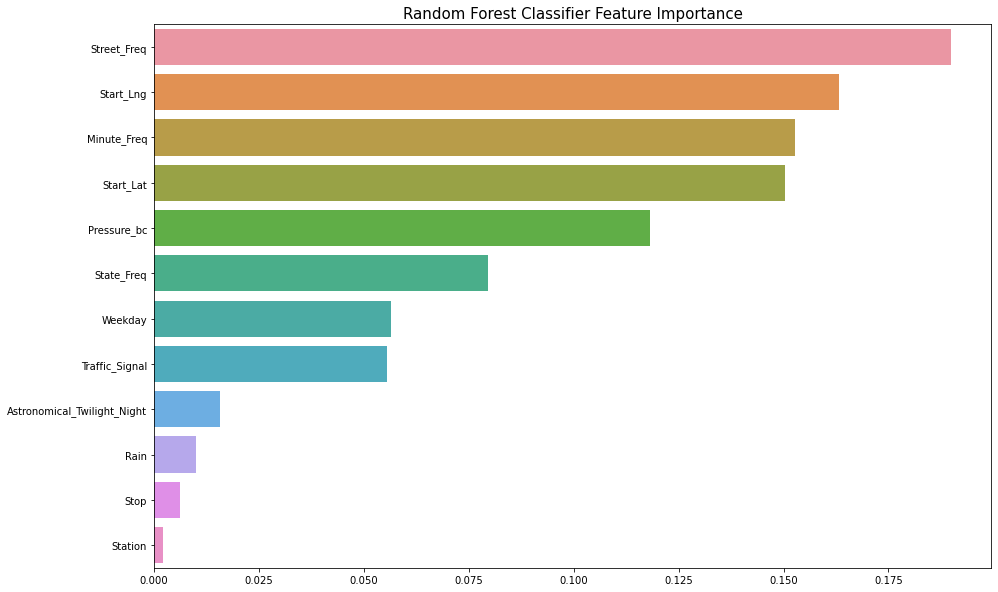
\includegraphics[width=130mm,height=\textheight,keepaspectratio]{images/rf_features.png}
    \caption{Random Forest Classifier Feature Importance}
    \label{fig:rf_features}
\end{figure}

\noindent
The 5 most important features it determined were:
\begin{enumerate}
    \item Street Frequency
    \item Start Longitude
    \item Minute Frequency
    \item Start Latitude
    \item Pressure (Box-Cox)
\end{enumerate}

I am not surprised that Street Frequency, Start Longitude, and Start Latitude were in the top 5. As seen in \cref{section:exploratory_analysis}, most severe accidents seemed to occur on interstate highways in densely populated regions (based on longitude and latitude). Along with the temporal input that the Minute Frequency feature provided, the pattern clearly indicates that severe accidents are likely to occur in the same location and time as severe accidents that have occurred in the past.

Unlike the other factors, I was surprised by the Pressure (Box-Cox) feature being so important. Since a strong negative correlation was found for this factor, I wonder if pressure plays an indirect role in causing severe accidents. This is unlikely to be due to the weather as none of the weather features like Rain seemed to have a strong correlation with severity. 

I was also surprised to see factors like Astronomical Twilight Night and Traffic Signal to only be somewhat important in predicting severe accidents as these are often cited as common dangerous driving conditions. As a further exploration, I would like to investigate these anomalies.

\newpage
\bibliography{ref}
\bibliographystyle{apalike}

\newpage
\appendix
\section{Appendix}
\label{section:appendix}

\subsection{Traffic Attributes}
\label{section:traffic_attrs}

\begin{longtable}[c]{l | l}
    Column & Description \\
    \hline
    ID & This is a unique identifier of the accident record. \\
    Source & Indicates source of the accident report. \\
    Severity & Shows the severity of the accident, a number between 1 and 4. \\
    Start Time & Shows start time of the accident in local time zone. \\
    End Time & Shows end time of the accident in local time zone. \\
    Start Latitude & Shows latitude in GPS coordinates of the start point. \\
    Start Longitude: & Shows longitude in GPS coordinate of the start point. \\
    End Latitude & Shows latitude in GPS coordinate of the end point. \\
    End Longitude & Shows longitude in GPS coordinate of the end point. \\
    Distance(mi) & The length of the road extent affected by the accident. \\
    Description & Shows natural language description of the accident. \\
\end{longtable}

\subsection{Address Attributes}
\label{section:address_attrs}

\begin{longtable}[c]{l | l}
    Column & Description \\
    \hline
    Number & Shows the street number in address field. \\
    Street & Shows the street name in address field. \\
    City & Shows the city in address field. \\
    County & Shows the county in address field. \\
    State & Shows the state in address field. \\
    Zip Code & Shows the zipcode in address field. \\
    Country & Shows the country in address field. \\
    Timezone & Shows timezone based on the location of the accident. \\
\end{longtable}

\subsection{Weather Attributes}
\label{section:weather_attrs}

\begin{longtable}[c]{l | l}
    Column & Description \\
    \hline
    Airport Code & Denotes the closest airport-based weather station. \\
    Weather Timestamp & Shows the time-stamp of weather observation. \\
    Temperature & Shows the temperature (in Fahrenheit). \\
    Wind Chill & Shows the wind chill (in Fahrenheit). \\
    Humidity & Shows the humidity (in percentage). \\
    Pressure & Shows the air pressure (in inches). \\
    Visibility & Shows visibility (in miles). \\
    Wind Direction & Shows wind direction. \\
    Wind Speed & Shows wind speed (in miles per hour). \\
    Precipitation & Shows precipitation amount in inches, if there is any. \\
    Weather Condition & Shows the weather condition. \\
\end{longtable}

\subsection{Point-Of-Interest Attributes}
\label{section:poi_attrs}

\begin{longtable}[c]{l | l}
    Column & Description \\
    \hline
    Amenity & Indicates presence of amenity in a nearby location. \\
    Bump & Indicates presence of speed bump or hump in a nearby location. \\
    Crossing & Indicates presence of crossing in a nearby location. \\
    Give Way & Indicates presence of give way sign in a nearby location. \\
    Junction & Indicates presence of junction in a nearby location. \\
    No Exit & Indicates presence of no exit sign in a nearby location. \\
    Railway & Indicates presence of railway in a nearby location. \\
    Roundabout & Indicates presence of roundabout in a nearby location. \\
    Station & Indicates presence of station (bus, train, etc.) in a nearby location. \\
    Stop & Indicates presence of stop sign in a nearby location. \\
    Traffic Calming & Indicates presence of traffic calming means in a nearby location. \\
    Traffic Signal & Indicates presence of traffic signal in a nearby location. \\
    Turning Loop & Indicates presence of turning loop in a nearby location. \\
\end{longtable}

\subsection{Period-of-Day Attributes}
\label{section:pod_attrs}

\begin{longtable}[c]{l | l}
    Column & Description \\
    \hline
    Sunrise Sunset & Shows the period of day based on sunrise/sunset. \\
    Civil Twilight & Shows the period of day based on civil twilight. \\
    Nautical Twilight & Shows the period of day based on nautical twilight. \\
    Astronomical Twilight & Shows the period of day based on astronomical twilight. \\
\end{longtable}

\subsection{Python Code for Data Processing, Analysis, and Visualization}
\label{code:python}
\pythoncode{main.py}

\end{document}
